Bitcoin has been largely unregulated till now. This has given free reign to the black market community and the underground network to use bitcoins for their shady deals. Unlike cash, bitcoin gives them the comfort of doing illegal activities without moving from their home. And unlike other methods of payment like banks and credit cards, bitcoin is anonymous in that the ownership of bitcoin cannot be directly traced back to a real person. This led to bitcoin being very appealing to criminals. Bitcoins have been used in drug deals, money laundering schemes and gambling. Bitcoin is also used for legitimate purposes with many merchants and online stores accepting the currency as payment. The diagram below shows briefly the events in the bitcoin world up to now.\\*

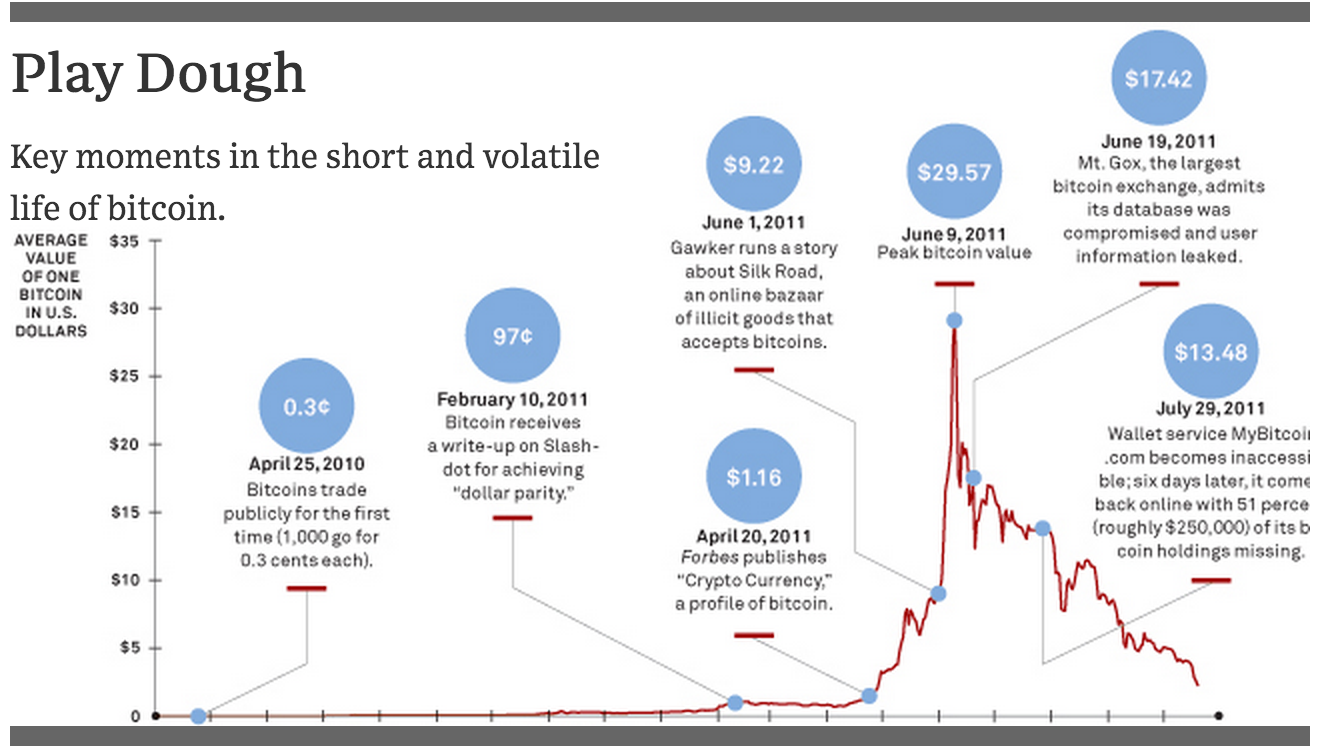
\includegraphics[scale=0.5]{images/life.png}

\section{Is Bitcoin really anonymous?}
The protocol behind bitcoin is designed to be a transparent system with the blockchain recording every transaction. Even though the transactions are known and the chain of ownership is known, the identity of the person possessing the bitcoin is not obvious. This has led people to argue that bitcoin is in fact  "pseudonymous" - meaning "false name", which allows people to use a disguised identity. Though there are various steps that a user can take to be careful, using bitcoin for illicit purchases is a bad idea even if the chain is anonymous. Jeff Garzik, a bitcoin core developer said, "Attempting major illicit transactions with bitcoin, given existing statistical analysis techniques deployed in the field by law enforcement, is pretty damned dumb."  What are these statistical analysis techniques that are being used to trace bitcoin transactions?

\section{How to get started with bitcoins?}
Users can get new bitcoins by mining (validating transactions on the block chain). But this activity requires a lot of computing power. So users usually join a mining pool like
"Deepbit" where they are paid proportionately according to the computing power they contribute \cite{deepbit}. The other option is to buy bitcoins by exchanging bitcoins for real
money. There are bitcoin exchanges where one can perform these transactions. Some popular bitcoin exchanges are Mtgox
\cite{mtgox}. Currently, one bitcoin costs about \$357.95. Once a user has the bitcoins, he stores them in a "wallet". A wallet is a software that stores the digital credentials for
your bitcoin holdings and allows you to spend them. Bitcoin-Qt \cite{qt} also called Satoshi Client was the first bitcoin wallet to be developed. One the user has the bitcoins in his wallet he can start spending them on goods and services.